\documentclass{article}\usepackage[]{graphicx}\usepackage[]{xcolor}
% maxwidth is the original width if it is less than linewidth
% otherwise use linewidth (to make sure the graphics do not exceed the margin)
\makeatletter
\def\maxwidth{ %
  \ifdim\Gin@nat@width>\linewidth
    \linewidth
  \else
    \Gin@nat@width
  \fi
}
\makeatother

\definecolor{fgcolor}{rgb}{0.345, 0.345, 0.345}
\newcommand{\hlnum}[1]{\textcolor[rgb]{0.686,0.059,0.569}{#1}}%
\newcommand{\hlsng}[1]{\textcolor[rgb]{0.192,0.494,0.8}{#1}}%
\newcommand{\hlcom}[1]{\textcolor[rgb]{0.678,0.584,0.686}{\textit{#1}}}%
\newcommand{\hlopt}[1]{\textcolor[rgb]{0,0,0}{#1}}%
\newcommand{\hldef}[1]{\textcolor[rgb]{0.345,0.345,0.345}{#1}}%
\newcommand{\hlkwa}[1]{\textcolor[rgb]{0.161,0.373,0.58}{\textbf{#1}}}%
\newcommand{\hlkwb}[1]{\textcolor[rgb]{0.69,0.353,0.396}{#1}}%
\newcommand{\hlkwc}[1]{\textcolor[rgb]{0.333,0.667,0.333}{#1}}%
\newcommand{\hlkwd}[1]{\textcolor[rgb]{0.737,0.353,0.396}{\textbf{#1}}}%
\let\hlipl\hlkwb

\usepackage{framed}
\makeatletter
\newenvironment{kframe}{%
 \def\at@end@of@kframe{}%
 \ifinner\ifhmode%
  \def\at@end@of@kframe{\end{minipage}}%
  \begin{minipage}{\columnwidth}%
 \fi\fi%
 \def\FrameCommand##1{\hskip\@totalleftmargin \hskip-\fboxsep
 \colorbox{shadecolor}{##1}\hskip-\fboxsep
     % There is no \\@totalrightmargin, so:
     \hskip-\linewidth \hskip-\@totalleftmargin \hskip\columnwidth}%
 \MakeFramed {\advance\hsize-\width
   \@totalleftmargin\z@ \linewidth\hsize
   \@setminipage}}%
 {\par\unskip\endMakeFramed%
 \at@end@of@kframe}
\makeatother

\definecolor{shadecolor}{rgb}{.97, .97, .97}
\definecolor{messagecolor}{rgb}{0, 0, 0}
\definecolor{warningcolor}{rgb}{1, 0, 1}
\definecolor{errorcolor}{rgb}{1, 0, 0}
\newenvironment{knitrout}{}{} % an empty environment to be redefined in TeX

\usepackage{alltt}
\usepackage{amsmath} %This allows me to use the align functionality.
                     %If you find yourself trying to replicate
                     %something you found online, ensure you're
                     %loading the necessary packages!
\usepackage{amsfonts}%Math font
\usepackage{graphicx}%For including graphics
\usepackage{hyperref}%For Hyperlinks
\usepackage[shortlabels]{enumitem}% For enumerated lists with labels specified
                                  % We had to run tlmgr_install("enumitem") in R
\hypersetup{colorlinks = true,citecolor=black} %set citations to have black (not green) color
\usepackage{natbib}        %For the bibliography
\setlength{\bibsep}{0pt plus 0.3ex}
\bibliographystyle{apalike}%For the bibliography
\usepackage[margin=0.50in]{geometry}
\usepackage{float}
\usepackage{multicol}

%fix for figures
\usepackage{caption}
\newenvironment{Figure}
  {\par\medskip\noindent\minipage{\linewidth}}
  {\endminipage\par\medskip}
\IfFileExists{upquote.sty}{\usepackage{upquote}}{}
\begin{document}

\vspace{-1in}
\title{Lab 05 -- MATH 240 -- Computational Statistics}

\author{
  Brendan Mariano \\
  Colgate  \\
  Mathematics  \\
  {\tt bmariano@colgate.edu}
}

\date{}

\maketitle

\begin{multicols}{2}
\begin{abstract}
In this lab, we used the \texttt{tidyverse} to group each artist and summarize their data for each song measuring feature. his allowed us to compare the similarity of each artist to Allentown for selected features and identify the primary contributor.
\end{abstract}

\noindent \textbf{Keywords:} Tidyverse; Summarizing; ggplot

\section{Introduction}
The overarching goal for this lab was to determine whether The Front Bottoms, Manchester Orchestra or All Get Out contributed most to their joint song Allentown. We had data from three different places: Essentia \citep{essentia}--a program that analyzes the sound of a track, additional Essentia models \citep{essentia_models}, and the LIWC, Linguistic Inquiry and Word Count \citep{liwc}, which provides features about the lyrics of a track. Our job was to determine two things which of the 160 features were relevant and to then analyze them in order to reach a conclusion about who contributed the most to Allentown. 
  The methods sections explains how we determined which features were relevant and how we presented them in an effective way. On the other hand, we convey the trends shown for each artist in the results section and analyze our findings to reach an overall conclusion in the discussion section. 


\section{Methods}
  Overall, the problem that we needed to solve was to determine who contributed most to the song. We had a collection of features from 10s of songs from each of the artists, however, we needed to summarize each of their data. This led us to using a summarize function, which created a table grouping each artist with all of their songs and analyzed their min, max, lower fence and upper fence for each quantitative feature. From here, we now had a table for comparison among artists for each feature. In order to translate this towards our overall goal, we determined whether Allentown's value for each feature was an outlier, out of the range or within the range. This allowed us to determine which features mattered and ultimately create plots displaying them.
  
  When choosing a feature, I ensured that at least one (often two) of the artists was not within range. This was because, if Allentown was within range for every artist, it wouldn't demonstrate any difference in individual contribution, which wouldn't help us to figure out who contributed more. There were 40 different features which fit our criteria, and it was at first difficult to choose. When deciphering were relevant, I researched what each of the features represented-- allowing me to select features that were dissimilar-- allowing for a more diverse set them. Lastly, I made sure to have four of the features be lyrical so that I was also analyzing the words rather than solely the sound of the music itself.
  
  To ultimately answer our question, we created plots to be used for analysis using ggplot2 \citep{ggplot2}. I found that box plots demonstrated my data effectively because they are easy to understand and I could insert a line indicating the Allentown value.
\section{Results}
  For the features related to the lyrical portion of the song, Cognition, Perception, power and Authentic, the Manchester Orchestra was the most similar to Allentown; they were within range for all four of the lyrical features while The Front Bottoms was only in range for two and All Get Out was only in range for one. This suggests that all of them contributed to the lyrical portion of Allentown, but Manchester Orchestra contributed the most. 
    For the features related to the sound of the song, the Manchester Orchestra continued to have the most features within its range. For instance, the Allentown value for \texttt{erbbands skewness}, which is otherwise known as the skewness of the error bands feature, is above the fence of All Get Out and the Front Bottoms, but within range of Manchester Orchestra. This suggests that Allentown has a right skewed distribution of error bands, meaning that they have more variation in higher frequencies which can be characteristic of songs by the Manchester Orchestra. Out of the eight different sound related features, Allentown was within range for the Manchester Orchestra every single time while it was only within range for All Get Out twice and zero times for The Front Bottoms.

   \begin{figure}[H]
    \begin{center}
       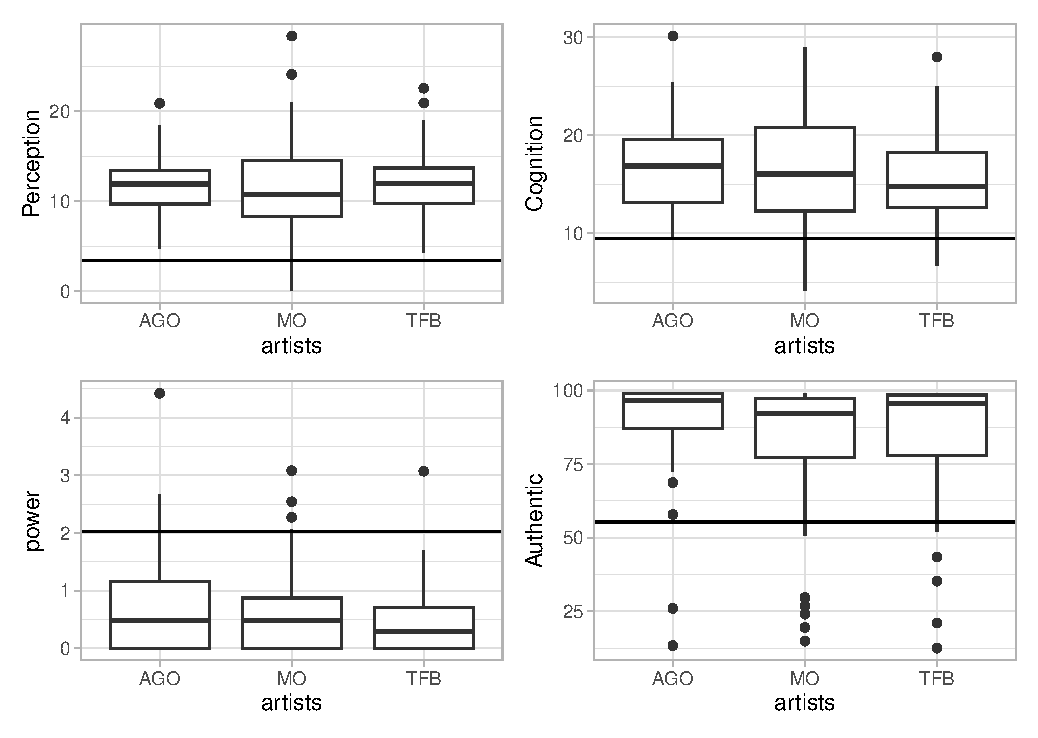
\includegraphics[scale=0.5]{lyrics.pdf}
       \caption{Plots features analyzing lyrics. FBO = The Front Bottoms, AGO = 
       All Get Out, MO = Manchester Orchestra}
     \label{lyrics_plot}
     \end{center}
   \end{figure}
   \begin{figure}[H]
    \begin{center}
       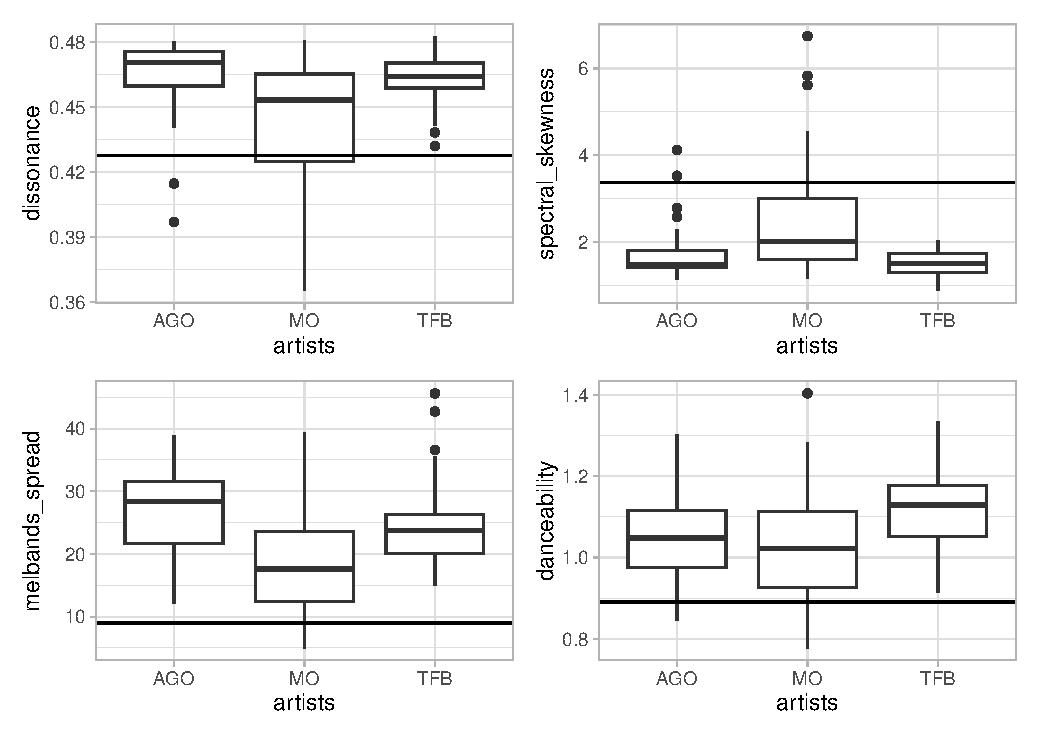
\includegraphics[scale=0.5]{sound1.pdf}
       \caption{Plots features analyzing sound. FBO = The Front Bottoms, AGO = 
       All Get Out, MO = Manchester Orchestra}
     \label{sound1}
     \end{center}
   \end{figure}
     \begin{figure}[H]
    \begin{center}
       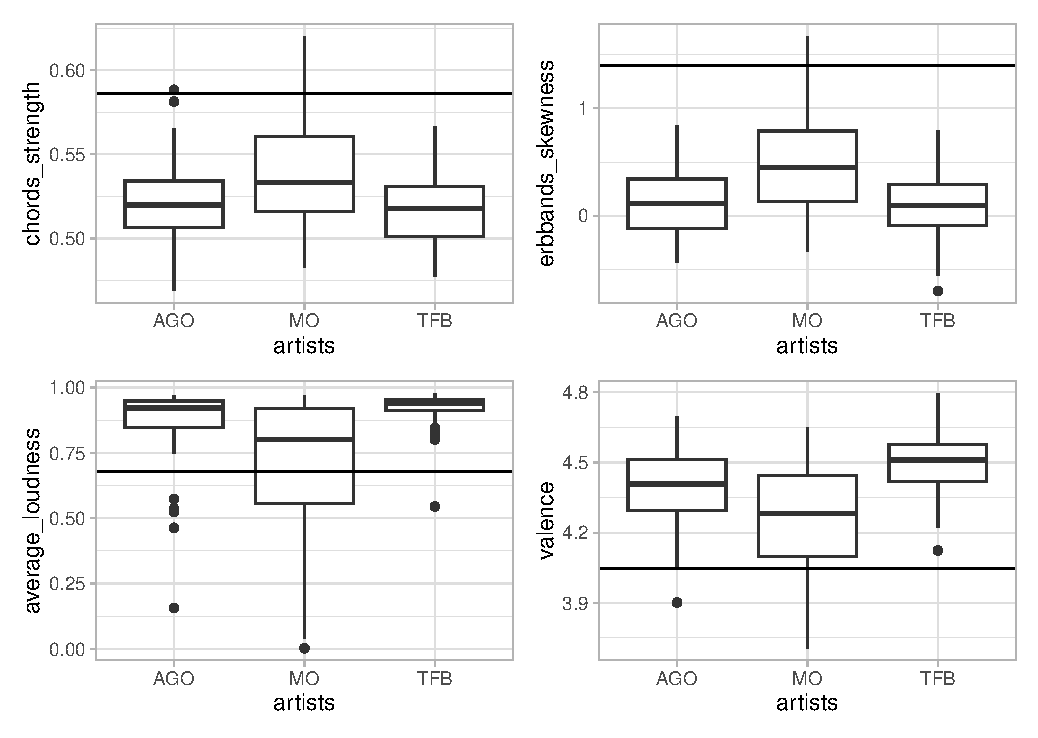
\includegraphics[scale=0.5]{sound2.pdf}
       \caption{Plots features analyzing sounds. FBO = The Front Bottoms, AGO = 
       All Get Out, MO = Manchester Orchestra}
     \label{sound2}
     \end{center}
   \end{figure}



\section{Discussion}
  In total, between the lyrical features and the production related features, Allentown was within the range of Manchester Orchestra 12 times while the The Front Bottoms was within range twice and All Get Out was within the range three times. This suggests that Manchester Orchestra contributed the most across all of portions of the song; however, since The Front Bottoms were within range for half of the lyrical features and none of the production related ones, it is likely that they contributed to the lyrical portion of the song. As for All Get Out, with two features within range out of eight for the production and one for lyrical out of four, it is likely that they contributed small amounts to different portions of the song.
  While 12 features seems like a small amount to reach  a conclusion, we researched the features significance so that they accurately represent the 40 features in which Allentown was not within range for at least one of the artists. Additionally, the 120 features which we didn't plot all had Allentown within range for each artist. Therefore, since we found the trend among the differing features, we can transfer our findings to the song overall. In this case, the Manchester Orchestra was within range for all of our selected features. Thus, they were the greatest contributor to Allentown.

%%%%%%%%%%%%%%%%%%%%%%%%%%%%%%%%%%%%%%%%%%%%%%%%%%%%%%%%%%%%%%%%%%%%%%%%%%%%%%%%
% Bibliography
%%%%%%%%%%%%%%%%%%%%%%%%%%%%%%%%%%%%%%%%%%%%%%%%%%%%%%%%%%%%%%%%%%%%%%%%%%%%%%%%
\vspace{2em}

\begin{tiny}
\bibliography{bib}
\end{tiny}
\end{multicols}

%%%%%%%%%%%%%%%%%%%%%%%%%%%%%%%%%%%%%%%%%%%%%%%%%%%%%%%%%%%%%%%%%%%%%%%%%%%%%%%%
% Appendix
%%%%%%%%%%%%%%%%%%%%%%%%%%%%%%%%%%%%%%%%%%%%%%%%%%%%%%%%%%%%%%%%%%%%%%%%%%%%%%%%
\newpage
\onecolumn
\section{Appendix}
\begin{table}[ht]
\centering
\begin{tabular}{rllll}
  \hline
 & The Front Bottoms & Manchester Orchestra & All Get Out & Feature \\ 
  \hline
1 & Out of Range & Within Range & Within Range & danceability \\ 
  2 & Out of Range & Within Range & Outlying & spectral\_skewness \\ 
  3 & Out of Range & Within Range & Out of Range & melbands\_spread \\ 
  4 & Out of Range & Within Range & Out of Range & erbbands\_skewness \\ 
  5 & Out of Range & Within Range & Outlying & dissonance \\ 
  6 & Outlying & Within Range & Outlying & average\_loudness \\ 
  7 & Out of Range & Within Range & Outlying & chords\_strength \\ 
  8 & Out of Range & Within Range & Within Range & valence \\ 
  9 & Within Range & Within Range & Outlying & Authentic \\ 
  10 & Outlying & Within Range & Within Range & power \\ 
  11 & Within Range & Within Range & Out of Range & Cognition \\ 
  12 & Out of Range & Within Range & Out of Range & Perception \\ 
   \hline
\end{tabular}
\caption{Summary of selected features}
\end{table}
\end{document}
